\documentclass[../_main/handlingar.tex]{subfiles}

\begin{document}
\motion{Stav till Entertainer}

Alla vet att på sektionen finns det en post som värderas lite över de andra, en post som ger glädje till
sektionen på ett sätt som ingen annan gör. En post som är sektionens olja till dess kedja, strömmen
till dess krets och sinusknutan till dess hjärta. Det är inte mer än rätt att denna post får någonting
som utmärker den mer än de andra. Krögarna har sitt svärd. Är det inte dags att Entertainern får
något att bära vid sin sida? Jag, som suttit på posten i ett år, tycker att det är hög tid. En Entertainer
ska alltid kunna underhålla, på studs. Direkt på begäran. Nästan trolla fram det kan man tycka. Men
vad vore en trollkarl utan sin stav? 


\begin{center}
    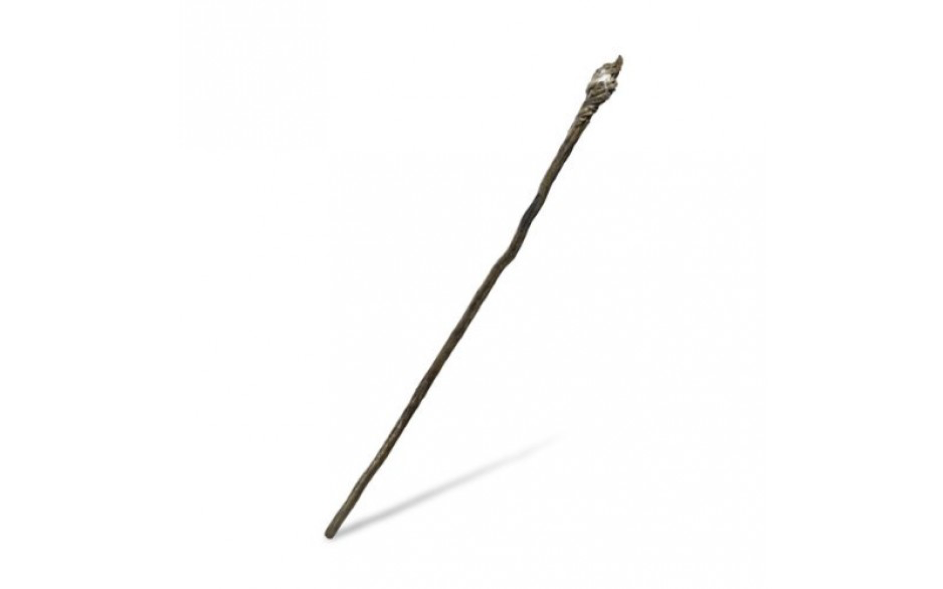
\includegraphics[width=10cm]{stav.png}
\end{center}

Därför yrkar jag
\begin{attsatser}
    \att avsätta 1899 kr till inköp av en 185 cm lång replika av Gandalfs stav från Sagan om Ringen,
    
    \att kostnaden belastar utrustningsfonden.

    \att Entertainern bär den här vid varje sektionsevent förutom under nollningen. (Det kan bli risk för
    stavkrig med Överphöset annars)

    \att det läggs på beslutsuppföljningen till HT2019 med sittande entertainer som ansvarig. 
\end{attsatser}

\begin{signatures}{1}
    \emph{I styrelsens tjänst}
    \signature{Adam Belfrage}{}
    
\end{signatures}

\end{document}
